% all comments have to begin at start of a line
% begin preamble
\documentclass[10pt]{article} 
\usepackage[utf8]{inputenc} 
\usepackage{amsmath}
\usepackage{graphicx}
\usepackage{lipsum}
\usepackage{biblatex}
\addbibresource{myref.bib}
\title{LaTeX Basic}
\author{Big-Taste-T}
\date{March 25, 2539}
% end preamble

% document section
\begin{document}

\maketitle
\section{Introduction}\label{sec:intr}
% observe how the new line is started \\
This is place-holer text.\\
Latex is a good tool.\\
Make it work for you.\\
\subsection{Background}
Latex was created a long time ago.\\
It still works good.~\cite[knuth:1984]\\
\\
There is a lot of stuff for it.\\
(\textbf{Bold Text})  (\textit{Italic Text})  (\underline{Underline Text})\\
\\
as discussed in \ref{sec:intr}
\\
the derivative of $x^2$ is $2x$\\
$$E=mc^2$$\\
\[E=mc^2\]
\\
As shown in Equation~\ref{eq:cube}
\begin{equation}\label{eq:cube}
    x^3
\end{equation}
\\
Area of a circle, Equation~\ref{eq:carea}
\begin{equation}\label{eq:carea}
    \pi r^2
\end{equation}

\begin{figure}[t]
    \centering
    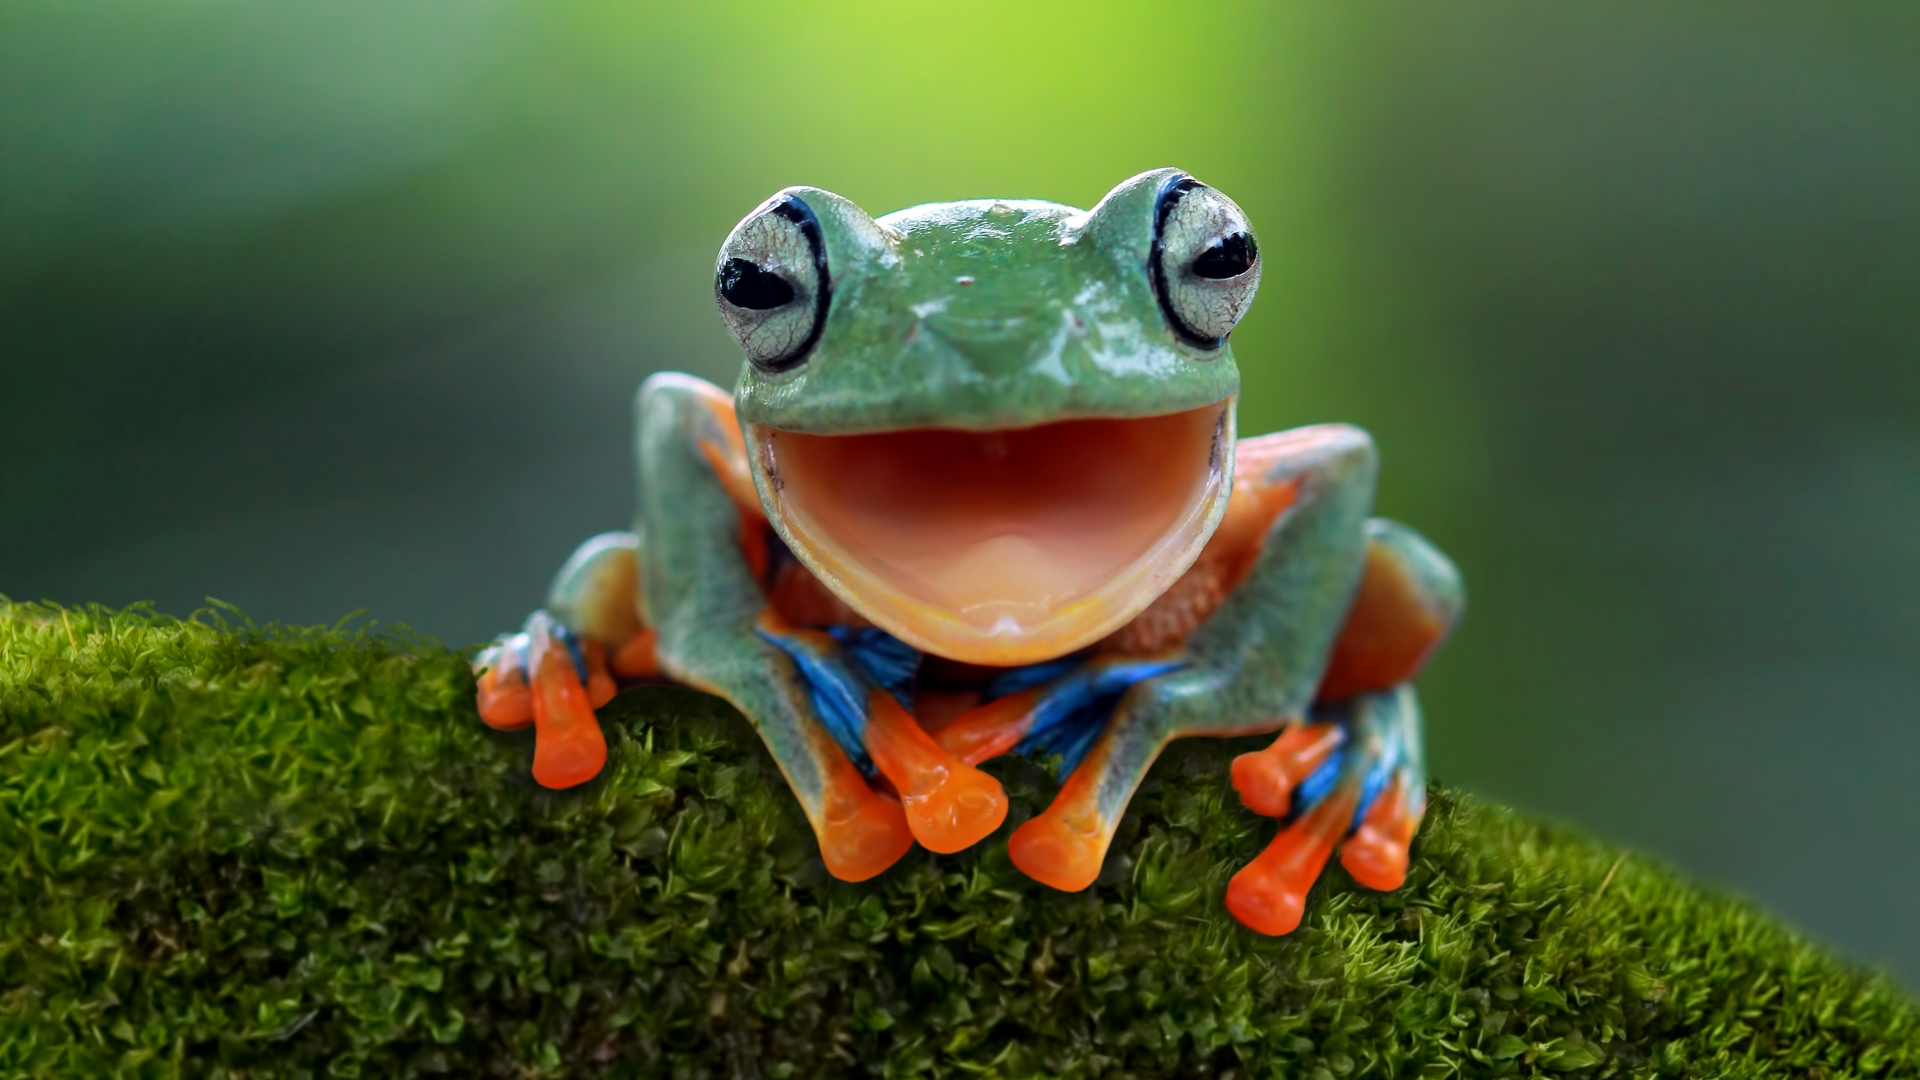
\includegraphics[width=\textwidth]{../ex1/frog}
    \caption{frog}
    \label{fig:myf}
\end{figure}

% try exporting a pandas df...
\begin{table}[]
    \centering
    \begin{tabular}{c|c}
        x & y \\
        ---&---\\
        0 & 0 \\
        1 & 1 \\
    \end{tabular}
    \caption{myt}
    \label{tab:myt}
\end{table}

\lipsum[2-2]

\begin{enumerate}
    \item bananas
    \item water
    \item eggs
\end{enumerate}

\begin{itemize}
    \item tent
    \item backpack
    \item shovel
\end{itemize}

\printbibliography[]

\end{document}
% close the document